\section{Redimensionando âmbitos (“ranges”)}

A verdadeira diversão começa quando você usa algumas UGens para controlar os parâmetros de outras UGens. O exemplo do theremin fez exatamente isto. Agora você tem todas as ferramentas para entender exatamente o que está acontecendo em um dos exemplos da seção \ref{sec:first-sine}. As três últimas linhas do exemplo demonstram passo a passo como o \texttt{LFNoise0} é usado para controlar a frequência:

\begin{lstlisting}[style=SuperCollider-IDE, basicstyle=\scttfamily\footnotesize]
{SinOsc.ar(freq: LFNoise0.kr(10).range(500, 1500), mul: 0.1)}.play;

// Separando em partes:
{LFNoise0.kr(1).poll}.play; // veja um simples LFNoise0 em ação
{LFNoise0.kr(1).range(500, 1500).poll}.play; // agora com .range
{LFNoise0.kr(10).range(500, 1500).poll}.play; // agora mais rápido
\end{lstlisting}

\subsection{Redimensione com o método \texttt{range}}
O método  \texttt{range} simplesmente redimensiona a saída de uma UGen. Lembre-se, \texttt{LFNoise0} produz números entre -1 e +1 (é uma UGen bipolar). Estes números brutos não seriam muito úteis para controlar frequência (precisamos de números perceptíveis na escala de audição humana). O \texttt{.range} pega esta saída entre -1 e +1 e a redimensiona entre qualquer valor mínimo e máximo que você fornecer como argumentos (neste caso, 500 e 1500). O número 10, que é o argumento para \texttt{LFNoise0.kr}, especifica a frequência da UGen: quantas vezes por segundos ele escolhe um novo número aleatório.

Resumindo: para usar a UGen para controlar algum parâmetro de outra UGen, primeiro você tem que saber qual o âmbito numérico que você quer. Os números serão frequências? Você os quer entre, digamos, 10 e 1000? Ou são amplitudes? Talvez você queira que as amplitudes estejam entre 0.1 (suave) e 0.5 (metade do máximo)? Ou você está tentando controlar o número de harmônicos? Você quer que ele esteja entre 5 e 19?

Uma vez que você sabe o âmbito que você precisa, use o método \texttt{.range} para fazer com que a UGen controladora faça a coisa certa.

Exercício: escreva uma linha de código simples que toca uma onda senoidal, cuja frequência é controlada por um \texttt{LFPulse.kr} (forneça agumentos apropriados para ele). Então, use o método \texttt{.range} para redimensionar a saída do \texttt{LFPulse} em algo que você queira escutar. 

\subsection{Redimensionando com \texttt{mul} e \texttt{add}}

Agora você sabe redimensionar a saída de UGens no servidor usando o método \texttt{.range}. A mesma coisa pode ser obtida em um nível mais fundamental usando os argumentos \texttt{mul} e \texttt{add}, que quase todos os UGens têm. O código abaixo mostra a equivalência entre as abordagens com \texttt{range} e de \texttt{mul/add}, ambos com uma UGen bipolar e uma UGen unipolar.

\begin{lstlisting}[style=SuperCollider-IDE, basicstyle=\scttfamily\footnotesize]
// Isso:
{SinOsc.kr(1).range(100, 200).poll}.play;
// …é o mesmo que isso:
{SinOsc.kr(1, mul: 50, add: 150).poll}.play;

// Isso:
{LFPulse.kr(1).range(100, 200).poll}.play;
// …é o mesmo que isso:
{LFPulse.kr(1, mul: 50, add: 100).poll}.play;
\end{lstlisting}

A figura \ref{fig:mul-add-scale} ajuda a visualizar como \texttt{mul} e \texttt{add} trabalham redimensionando as saídas de UGens (um \texttt{SinOsc} é usado como demonstração).

\begin{figure}[h!]
\centerline{\framebox{
	\includegraphics[scale=0.6]{fig-mul-add-scale.pdf}}}
\caption{Redimensionando âmbitos de UGens com mul e add}
\label{fig:mul-add-scale}
\end{figure}

\subsection{\texttt{linlin} e seus amigos}

Para qualquer outro redimensionamento arbitrário de âmbitos, você pode usar os práticos métodos \texttt{linlin}, \texttt{linexp}, \texttt{explin} e \texttt{expexp}. Os nomes nos métodos dão uma dica do que eles fazem: converter um âmbito linear em outro âmbito linear (\texttt{linlin}), linear para exponencial (\texttt{linexp}), etc.

\begin{lstlisting}[style=SuperCollider-IDE, basicstyle=\scttfamily\footnotesize]
// Um punhado de números
a = [1, 2, 3, 4, 5, 6, 7];
// Redimensione para 0-127, linear para linear
a.linlin(1, 7, 0, 127).round(1);
// Redimensione para 0-127, linear para exponencial
a.linexp(1, 7, 0.01, 127).round(1); // não use zero para um âmbito exponencial
\end{lstlisting}

Para uma revisão acerca de linear e exponencial, procure online a diferença entre progressões aritméticas e geométricas. Brevemente, sequências lineares (aritméticas) são como "1, 2, 3, 4, 5, 6" or "3, 6, 9, 12, 15", etc; e sequências exponenciais (geométricas) são como "1, 2, 4, 8, 16, 32" or "3, 9, 27, 81, 243", etc.



